\chapter{Concept}
\label{Concept}

This chapter covers the development of a concept, usable for the navigation for a mobile platform. 

The selection of navigation stacks is quite sparse. Especially considering the defined requirements. In general when it comes to navigation there are only two well documented stacks based on ROS to choose from.

\begin{itemize}
	\item navigation\_stack
	\item MoveIt
\end{itemize}

In contrast to the navigation\_stack MoveIt is largely used for the path planning and navigation of industrial robot arms and therefore not suited for this application.

The navigation\_stack provides a general setup proposal which seems to be a good starting point for robot navigation, but it has multiple parts that need be modified to adhere to the defined requirements.

\begin{figure}[H]
	\centering
	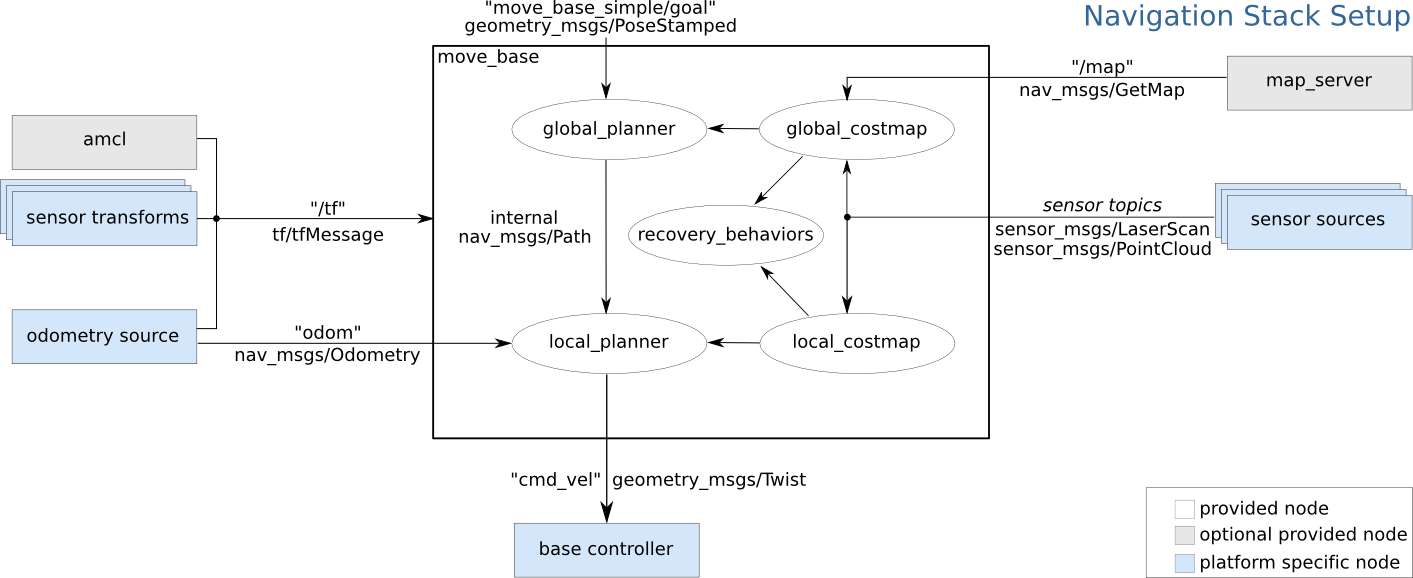
\includegraphics[width=\textwidth]{Pictures/navigation stack setup}
	\caption{navigation stack setup\cite{movebase}}
	
	\label{navigation stack setup}
\end{figure}


\section{platform specific nodes}
Since the platform specific nodes are unique to each robot these will need to be adjusted.\\
\subsection{sensor sources}

The following sensors will be predefined for this concept:

\begin{itemize}
	\item lidar
	\item wheel encoder
	\item imu
	\item camera
\end{itemize}

Since these sensors will certainly have noise we firstly need to add additional filters for the sensor signals. 



\subsection{Odometry source}
The odometry is all ways a result of sensor data. Therefore we can make a direct connection between the sensor filters and the odometry input. These Filters will also feature nodes that transform the incoming sensor data into a useable format.

\subsection{Sensor transforms}
To know the position of every sensor relative to the robot and his odometry the tf\_tree has to be build. While this can be realized using static transform publishers there is also a cleaner way using the ros package robot\_state\_publisher. It then requires a robot description in URDF format that specifies the relations between everything mounted on the robot.
The transformation between the base of the robot and the odom will be build by the filtered odometry.

The remaining platform specific nodes are all available since the simulated robot will be used and provides a motor controller, as well as all of the sensors and data sources.

\section{SLAM}

The map is a representation of the robots environment. If this is known from the start it is known, where the robot can go and where not.\\
 In this scenario the robot will always start blind, meaning it will not know anything about its surrounding other than that it can expect a road to be somewhere, which makes the map\_server of the navigation\_stack and its functionality to convert prerecorded maps redundant.\\
Adding to that amcl (the localization package of the navigation\_stack) will no longer work since it tries to find a position in a predefined map based on the current sensor signals.\\
Knowing the environment and the position of the robot in it is an important part in robot navigation since it allows to send goals that are relative to the environment and not to the robot. That is why the usage of a SLAM algorithm becomes highly useful. This node supplies both the current map and the position of the robot in it.\\
The big improvement this concept has from SLAM is, that goals could be extracted from the map, instead of being estimated after the first round on the track.

This node will publish the transform between the map and the odom frame so the position of the robot and every sensor signal can be determined relative to the map frame.\\

Unfortunately the data that can be fed to the SLAM node is very limited, since it is not guaranteed, that the lidar all ways sees static obstacles. An other data source for the SLAM algorithm could be the points extracted from the road detection. The problem with these is, that they don't have a lot of features in them other than the corridor like point distribution which.\\

This significantly decreases the reliability of the map which therefore will highly depend on good odometry.

To get the best map both of the data inputs have to be used, which results in the need of a SLAM algorithm with multiple inputs.\\

\section{Provided nodes}

The provided nodes do not have to be reordered but the recovery behaviors will be removed. These will be incorporated in the incoming goals instead.

To define the tasks of the nodes of move\_base they will be sepparated into two sections a global and a local stage, each of the stages consists out of a planner and a costmap.\\
\subsection{global stage}
The general task of the global planner is like described in the theoretical knowledge to plan a rough path through the grid that will not collide with any obstacle.\\

In this scenario the global planner will be required to guide the robot on the correct lane as well. This results in two additional requirements:

\begin{itemize}
	\item the global costmap needs to incorporate cost that set a preference for the right lane but allow the global path to go to the left in case of a blockage
	\item the global planner has to respect not only lethal but every cost
\end{itemize}

\subsection{local stage}
The local stage on the other hand has the task of finding a for the kinematic of the robot feasible path that does not collide with objects.\\
This Path needs to be close to the global path and follow the lane changes dictated by the global stage but it needs to be able to separate itself from the global path if necessary.

\section{PoseFinder}
The job of this node is to extract the pose of a goal from the sensor data or the map (if available).\\

The requirements of this node will be defined in the "Configuration and testing" section
\section{sensor filter}
Here the entire data processing takes place, which converts the sensor data into a usable format. This block in the concept consists out of the following nodes:

\begin{itemize}
	\item \textbf{road\_detection} will extract approximated polynomials for the road markings and the lanes from the camera data.
	\item \textbf{markfreespace} needs to publish points that need to be inflated to generate restricted areas in the costmap. Also produces combined data of the road\_detection and the lidar for SLAM.
	\item \textbf{laser\_filter} removes error points at the edges of obstacles
	\item \textbf{robot\_localization} improves the odometry by fusing wheel encoder data and imu data
\end{itemize}

The road\_detection and the markfreespace nodes are obligatory while the two remaining ones need to be implemented to improve the usability of the data of exactly this setup and might not be needed on a different robot

\section{Resulting concept}
The following simplified schematic is the concept of the navigation stack setup. Not all of the connections between the nodes will be highlighted, to keep schematic simple.\\

\begin{figure}[h!]
	\begin{center}
		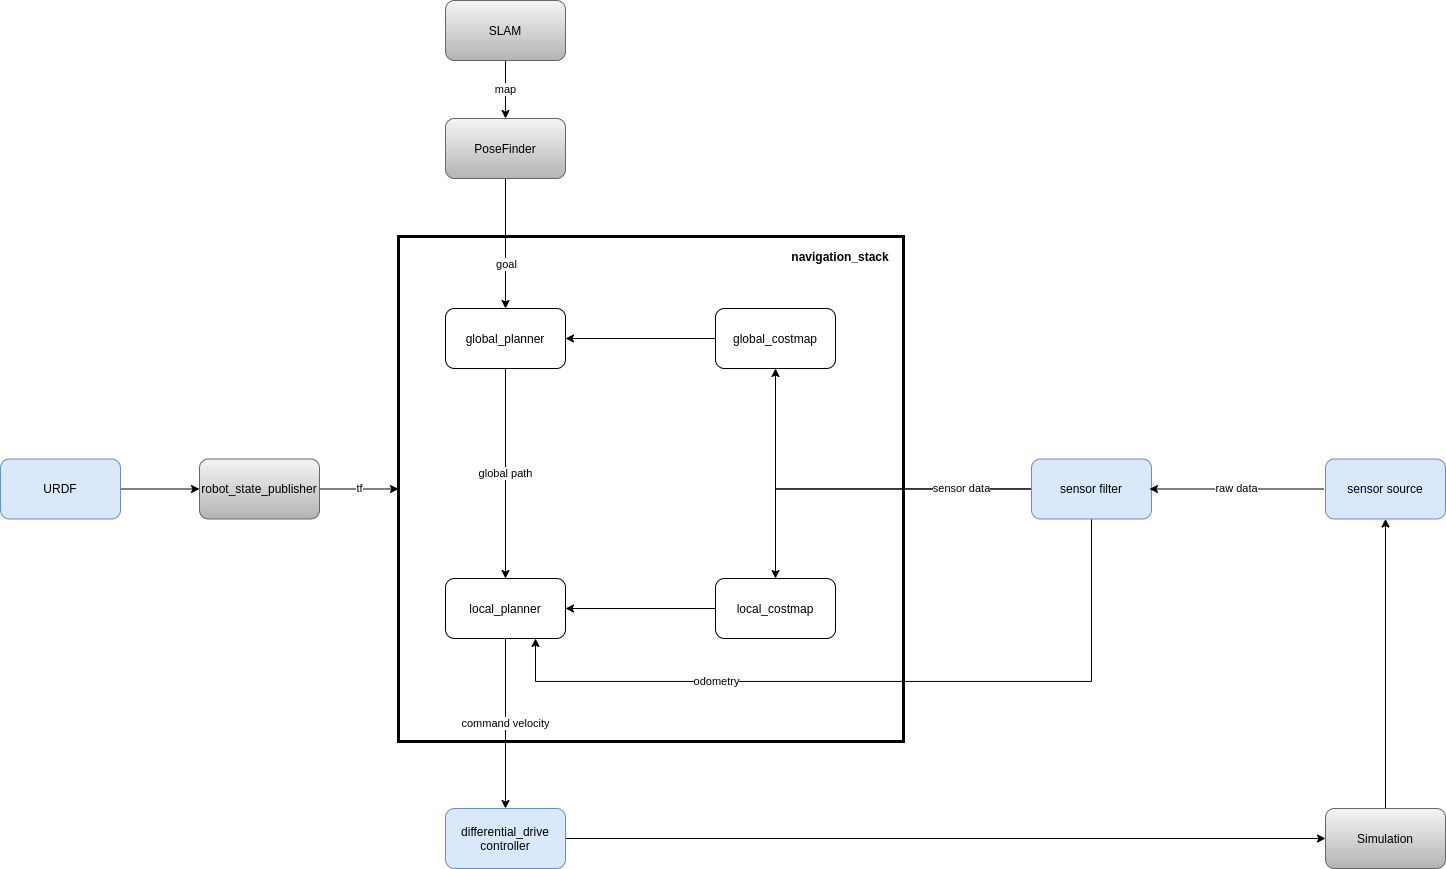
\includegraphics[width=140mm]{Pictures/Updated navigation concept}
		\caption[Updated navigation concept]{Updated navigation concept}
	\end{center}
\end{figure}



The PoseFinder will first find a goal based on the current state of the map and the sensor data and sends it to the navigation stack. This then uses the filtered sensor data to determine, where the robot is, where it is allowed to go and where not. The cascading planners then determine first a rough, collision free, path on the correct lane and then a path that is possible for the kinematics of the robot. This path then gets converted to velocity commands and sent to the differential drive controller.\\
This procedure will be repeated at a configurable frequency so the robot will never reach its finish. This is necessary since it is unknown if the goal, in the space that has not been explored yet, is perfectly on the future road, or if it is in an obstacle.




